%------------------------------------------------------------------------------
\begin{frame}
  \frametitle{Cas des cables et des blindages}
  \begin{columns}[T]
    \column{0.5\linewidth}
    \begin{itemize}
      \item Blindage de r\'er\'erence $w_0$ et $N^1$ conducteurs $w_1 \cdots w^1_N$
      \item Chaque conducteur $w_i$ a $NN_i$ sous conducteurs dedans
      \item Chaque conducteur $w_i$ matrice d'inductance $L_{int}^i$
      \item $L_{ext}$ : matrice d'inductance des conducteurs ext\'erieurs  
    \end{itemize}
    \column{0.5\linewidth}
    \begin{center}
      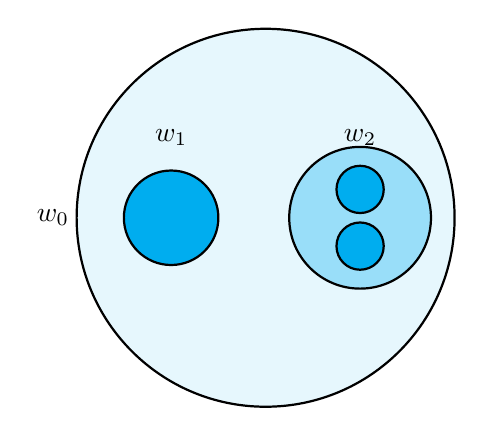
\begin{tikzpicture}[scale=0.6]
        \draw [thick,fill=cyan!10!white]  (0,0) node (v1) {} ellipse (4 and 4);
        \node at (-4.5,0) {$w_0$};
        \draw [thick,fill=cyan] (-2,0) ellipse (1 and 1);
        \draw [thick,fill=cyan!40!white] (2,0) ellipse (1.5 and 1.5);
        \node at (-2,1.7) {$w_1$};
        \node at (2,1.7) {$w_2$};

        %      \draw [thick,fill=cyan] (2,0) ellipse (0.5 and 0.5);
        \draw [thick,fill=cyan] (2,0.6) ellipse (0.5 and 0.5);
        \draw [thick,fill=cyan] (2,-0.6) ellipse (0.5 and 0.5);
      \end{tikzpicture}
    \end{center}
  \end{columns}
\end{frame}
%------------------------------------------------------------------------------


%------------------------------------------------------------------------------
\begin{frame}
\frametitle{Cas des cables et des blindages}
On obtient
\[ \left[ \begin{array} {c}
\phi_{ext} \\
\tilde{\phi}^1_{int}  \\
\vdots \\
\tilde{\phi}^{N_{int}}_{int} \end{array}  \right]  = 
\left[ \begin{array} {cccc}
L_{ext} & & & \\
  & L^1_{int}& &  \\
 & &\ddots &  \\
 & & & L^{N_{int}}_{int} \end{array}  \right]
 \left[ \begin{array} {c}
\tilde{I}_{ext} \\
I^1_{int}  \\
\vdots \\
I^{N_{int}}_{int} \end{array}  \right] 
\] \\[0.6cm]
en d'\'eduite
\[ \left[ \begin{array} {c}
\phi_{ext} \\
\tilde{\phi}_{int} \end{array}  \right]  = 
\left[ \begin{array} {cc}
L_{ext} & \\
  & L_{int}  \end{array}  \right]
 \left[ \begin{array} {c}
\tilde{I}_{ext} \\
I_{int} \end{array}  \right] 
\] \\[0.6cm]
($\tilde{\phi}_{int}$ potentiel int\'erieux calcul\'e avec une r\'ef\'erence sur les blindages)
\end{frame}
%------------------------------------------------------------------------------


%------------------------------------------------------------------------------
\begin{frame}
\frametitle{Cas des cables et des blindages}
Changement de variables
\begin{equation}
\phi_{int} = \tilde{\phi}_{int} +\delta^T \phi_{ext},
\end{equation}
avec $\delta$ : matrice de taille $N_{ext}\times N_{int}$ et
\begin{equation}
\delta(i,j)=
\begin{cases}
1 \qquad \text{si le conducteur $j+N_{ext}$ est dans le conducteur $i$,} \\
0 \qquad \text{sinon.}
\end{cases}
\end{equation}
De plus, 
\begin{equation}
\phi_{ext} = L\tilde{I}_{ext}=L(I_{ext}-\delta I_{int})
\end{equation}
La matrice d'inductance globale
\[ \left[ \begin{array} {c}
\phi_{ext} \\
\phi_{int} \end{array}  \right]  = 
L
 \left[ \begin{array} {c}
I_{ext} \\
I_{int} \end{array}  \right] 
\] 
avec
\[ L = P_I^T \left[ \begin{array} {cc}
L_{ext} &0 \\
0 & L_{int} \end{array}  \right] P_I , \qquad 
P_I
\left[ \begin{array} {cc}
1 & -\delta \\
0 & 1 \end{array}  \right]
 \] 

\end{frame}
%------------------------------------------------------------------------------
